\subsection*{Træning} \label{sec:traening}
Brugeren har mulighed for at foretage træninger baseret på forskellige træningsformer og træningstyper. Derudover skal træningen kunne tilpasses individuelt under hver enkelt træningssession, samt tilkoble kompatible måleenheder for at opnå en vejledende træning.  
Aktivitetsdiagrammet over træningen fremgår af \autoref{fig:traening}. 

\begin{figure} [H]
\centering
\textbf{Aktivitetsdiagram: Træning}\par\medskip
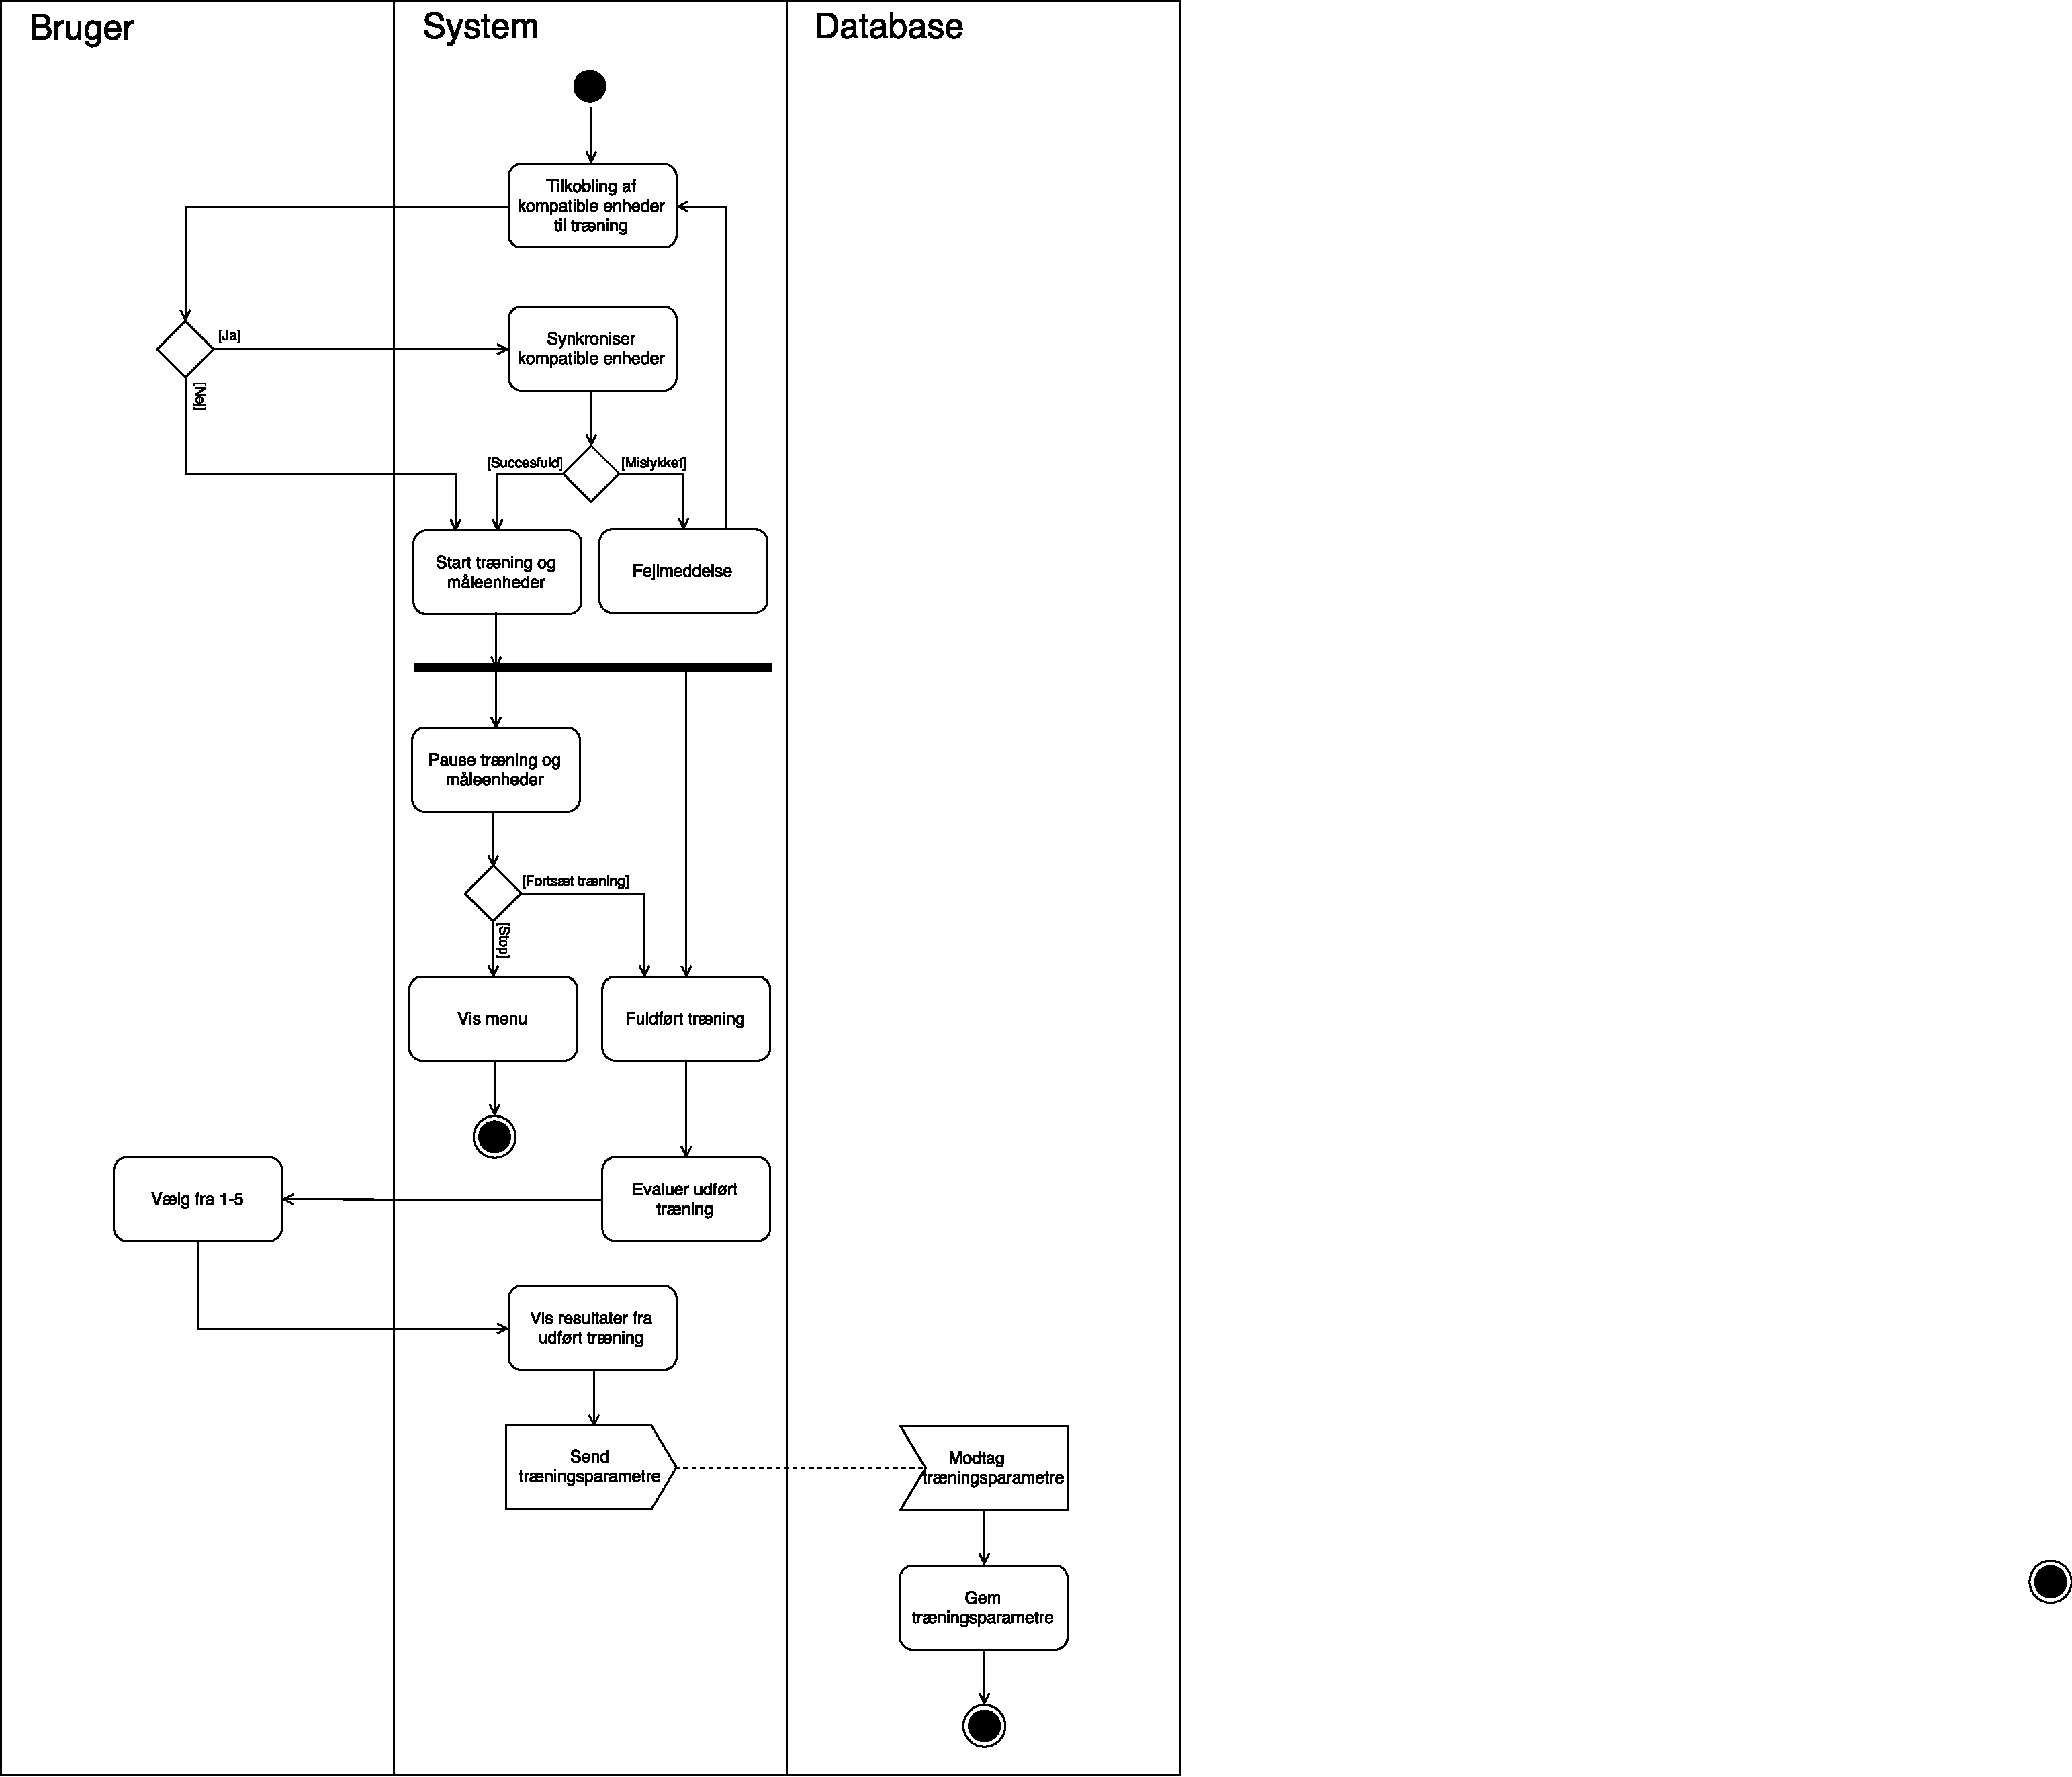
\includegraphics[width=0.8\textwidth]{figures/aktivitetsdiagram/Traening}
\caption{Aktivitetsdiagram over træning. Tilpasning af træningsniveau uddybes af \autoref{fig:traeningsniveau}.}
\label{fig:traening}
\end{figure}

\noindent
Før selve træningen påbegyndes, skal brugeren angive den ønskede træningsform, herunder konditions-, styrketræning eller vejrtrækningsøvelser. Ud fra den valgte træningsform skal brugeren angive træningstype, eksempelvis kan der ved valg af konditionstræning vælges gå, løbe eller cykle. Træningsniveau skal efterfølgende tilpasses. Tilpasning af træningsniveauet er  yderligere beskrevet af \autoref{fig:traeningsniveau}. Når systemet har tilpasset træning, tjekker systemet automatisk om der er kompatible måleenheder, hvis dette er tilfældet tilkobles disse. Ellers kan træningen påbegyndes uden. Brugeren starter herefter træningen og grænsefladen for denne vises. Under træningen vil systemet kontinuert vise træningen og målinger, der foretages. Brugeren kan til en hver tid vælge at afslutte træningen, dog skal denne handling bekræftes i tilfælde af, at brugeren ved en fejl angiver, at træningen skal stoppes. 
Ved bekræftelse stopper systemet træningen og afventer, at brugeren giver en evaluering. Efter evalueringen sendes evaluering og træningsresultater til en database, hvor det gemmes.


\subsubsection*{Tilpasning af træningsniveau} \label{sec:traeningsniveau}
Tilpasning af træningsniveau er en funktion der skal tage højde for daglige variationer ved at anbefale et træningsniveau ud fra brugeres kategorisering, daglige helbredstilstand og tidligere evalueringer af træninger.  
Aktivitetsdiagrammet over tilpasning af træningsniveau fremgår af \autoref{fig:traening}.
 
\begin{figure} [H]
\centering
\textbf{Aktivitetsdiagram: Tilpasning af træning}\par\medskip
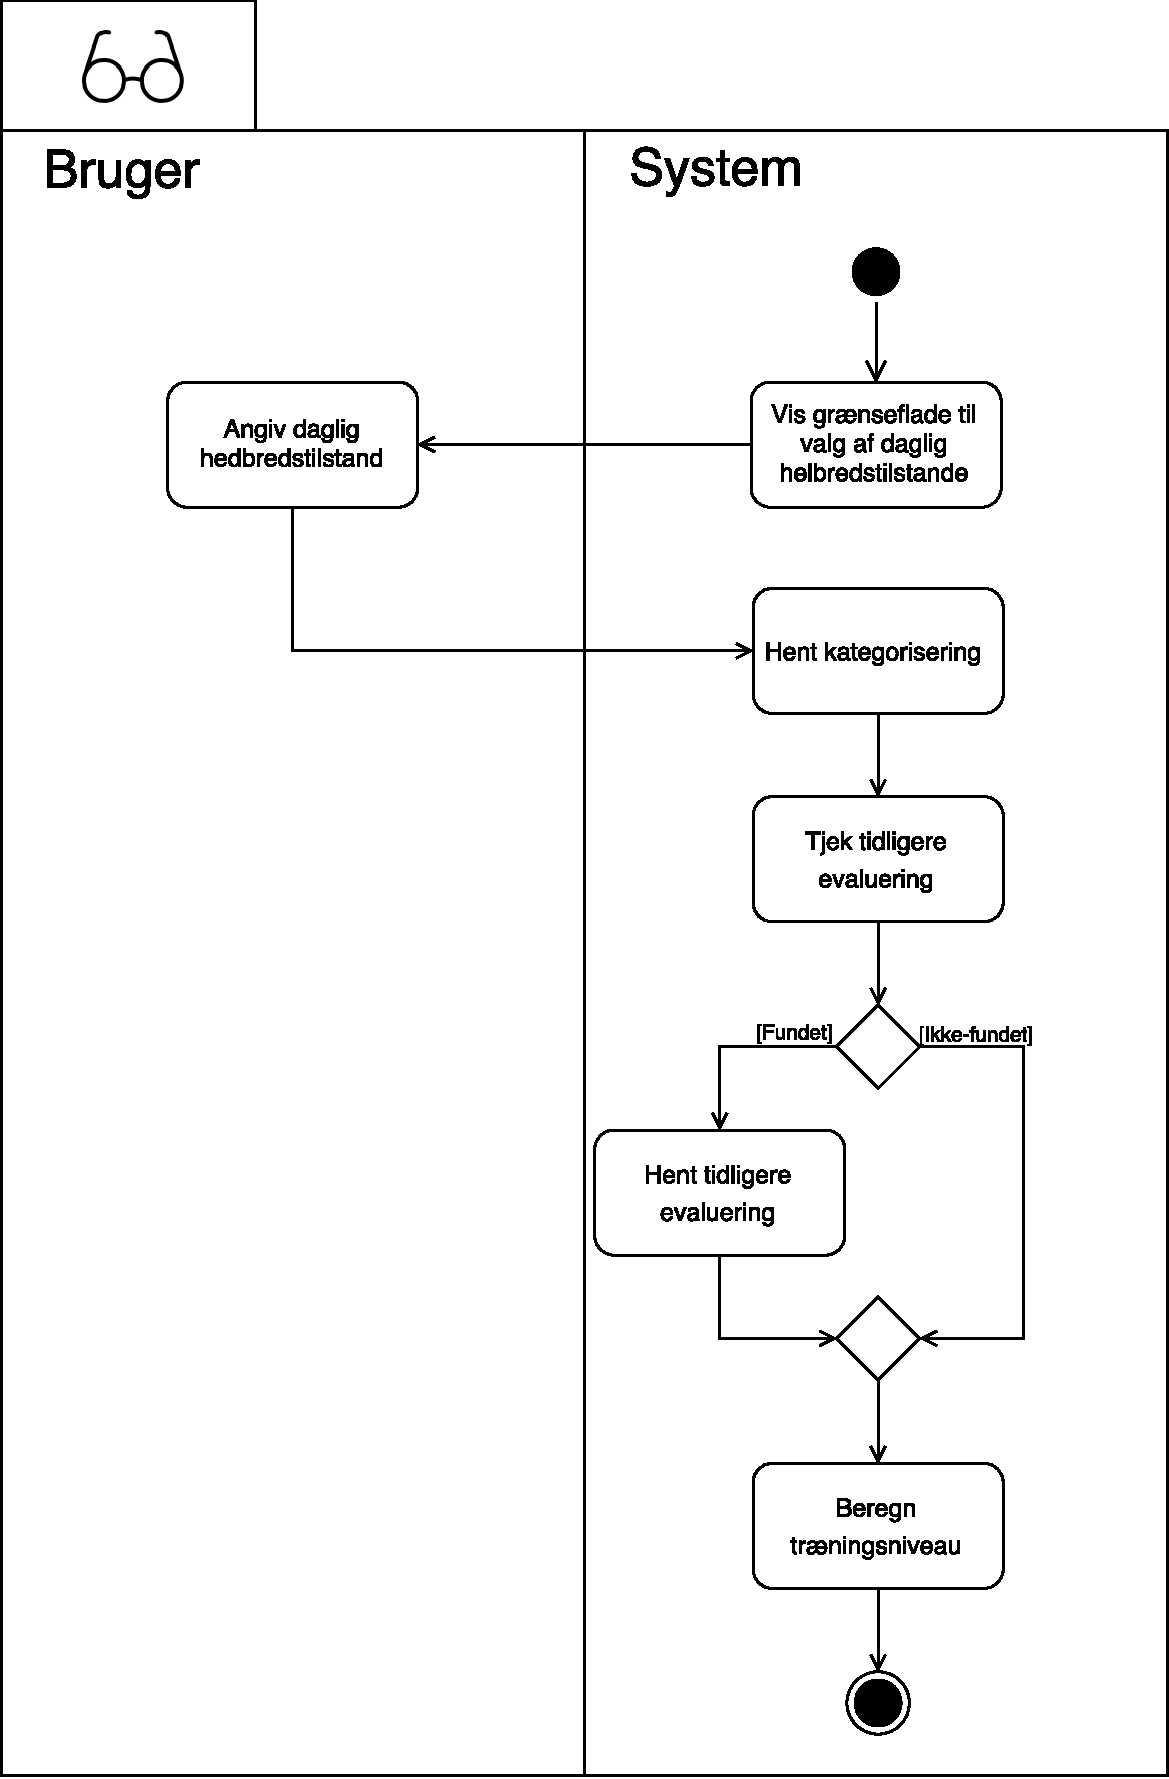
\includegraphics[width=0.8\textwidth]{figures/aktivitetsdiagram/Tilpasningaftraeningsniveau}
\caption{Aktivitetsdiagram over tilpasning af træningsniveau.}
\label{fig:traeningsniveau}
\end{figure}

\noindent
For at systemet kan tilpasse træningsniveauet vises grænsefladen for valg af daglig helbredstilstand, hvortil brugeren skal angive sin helbredstilstand. Systemet henter kategorisering og tjekker om der er tidligere evalueringer for den valgte træningsform og -type. Hvis brugeren ikke har angivet tidligere evalueringer bestemmes niveauet ud fra resterende parametre. Hvis de findes hentes de tidligere evalueringer. Tilpasningen af træningsniveau beregnes efterfølgende. Et simpel eksempel på denne beregning fremgår af \autoref{tab:beslutningstabel}. Tabellen beskriver hvordan en algoritme, ville regulere træningsniveauet, således der tages højde for den enkelte bruger.

\begin{table}[H]
\centering
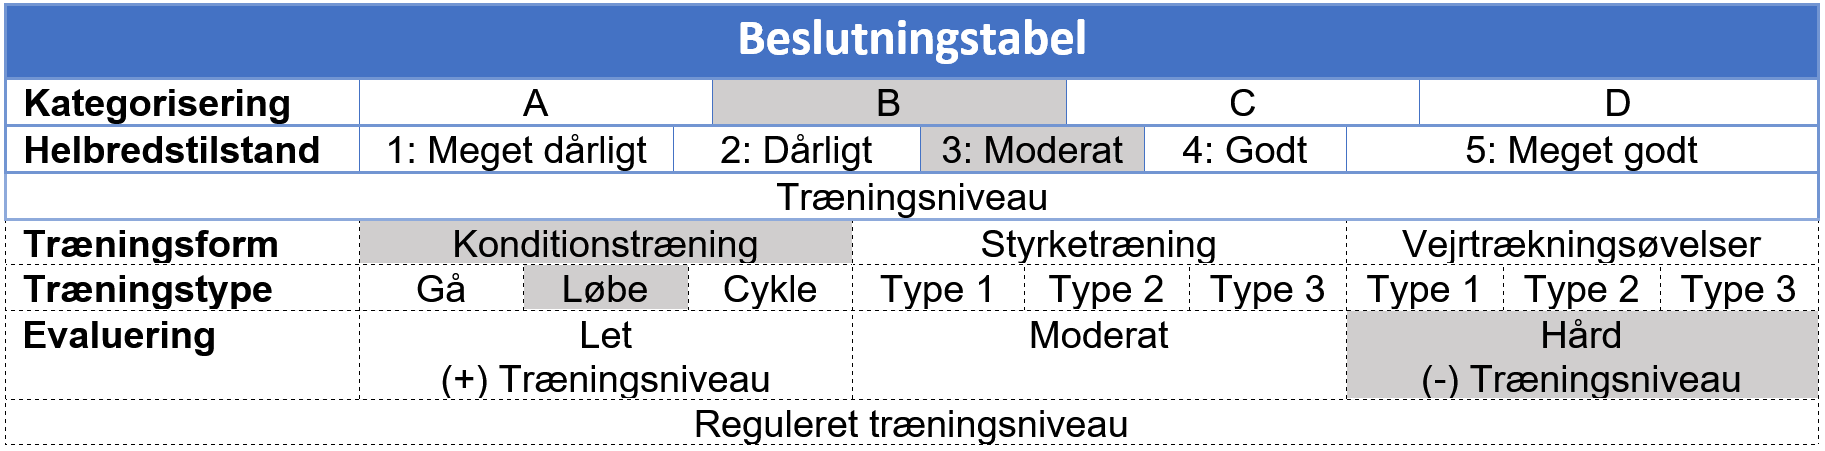
\includegraphics[width=1\textwidth]{figures/aktivitetsdiagram/beslutningstabel}
\caption{Beslutningstabel for træningsniveau. Kategorisering, daglig helbredstilsand samt eventuel evaluering anvendes til at bestemme træningsniveauet til den enkelte bruger. Af dette eksempel er brugeren kategoriseret B med en helbredstilstand, der er angivet som moderat. Dertil har brugeren valgt løb under konditionstræning. Tidligere har brugeren haft samme daglig helbredstilstand samt træning, og evalueret denne træning som værende hård. Dette muliggøre en regulering af træningsniveauet fra sidste træning, hvorfor niveauet i dette tilfælde sænkes.}
\label{tab:beslutningstabel}
\end{table} 

\noindent
Af \autoref{tab:beslutningstabel} fremgår en simpel beslutningstabel for, hvorledes et træningssæt tilpasses den enkelte bruger. Beslutningstabellen tager udgangspunkt i brugerens kategorisering, daglig helbredstilstand samt en eventuel evaluering. Brugeren er i dette tilfælde kategoriseret til B. Helbredstilstanden angives førend en træning påbegyndes, for således at tilpasse niveauet til den pågældende dag. Helbredstilstanden angives efter \textit{1: Meget dårligt}, \textit{2: Dåligt}, \textit{3: Moderat}, \textit{4: Godt} eller \textit{5: Meget godt}, hvortil brugerens helbredstilstand her angives som moderat.
Træningsniveauet vurderes dermed ud fra brugerens kategorisering samt helbredstilstand. 
For at have mulighed for at kunne regulere træningssættet yderligere, medregnes den forhenværende evaluering, der er forbundet med samme helbredstilstand, træningsform og type. I dette tilfælde har brugeren før haft samme helbredstilstand, træningsform samt type og dertil evalueret denne træning til værende hård. Algoritmen regulerer hertil træningsniveauet for denne træning ned, for således at give brugeren en bedre og mere tilpasset træningsoplevelse. 
